This example illustrate how to use BFilt for continuous-discrete filtering. Here the state is described by the following linear stochastic differential equation : \[ d \left ( \begin{array}{c} x \\ \dot{x} \\ \end{array} \right ) = \left ( \begin{array}{cc} 0 & 1 \\ -w_0^2 & -\gamma \\ \end{array} \right ) \left ( \begin{array}{c} x \\ \dot{x} \\ \end{array} \right ) dt + \left( \begin{array}{c} 0 \\ b \\ \end{array} \right ) dt + \left ( \begin{array}{c} 0 \\ g \\ \end{array} \right ) dW(t) \]

Where W(t) is a Wiener process,

$ w_0^2=16, \gamma = 2, b=8, g=2$ and the initials conditions $ X_0=(0,0) $ and $ R_0=diag[0,3]$.

The state $ X(t) = (x,\dot{x})(t)$ is then observed by the output $ Y_k \in \mathcal{R} $ : \[ Y_k = x(t_k) + V_k \]

at discrete time $ t_k $. The sampling period $ T_s = t_{k-1} - t_k = 0.2s $ and $ V_k \sim \mathcal{N}(0,0.001) $. In fact only the position is observed. First this model must be define as a sister class of linear time invariant continuous discrete models (\hyperlink{class_linear___c_d___model}{Linear\_\-CD\_\-Model}). 

\begin{DocInclude}\begin{verbatim}#ifndef __ORNSTEIN_UHL__
#define __ORNSTEIN_UHL__

#include <bfilt/gaussian_model.h>

class Ornstein_Uhlenbeck_Model : public Linear_CD_Model
{
public :
      double gamma;
      double w;
      double b;
      double g;
      Ornstein_Uhlenbeck_Model(void);


};

#endif
\end{verbatim}
\end{DocInclude}
 The \hyperlink{class_linear___c_d___model}{Linear\_\-CD\_\-Model} are implemented in the following form : \[ dX(t) = A X(t)dt + Bdt + C dW(t) \] \[ Y_k = H X(t_k) + h + V_k \] The constructor of Ornstein\_\-Uhlenbeck\_\-Model is then : 

\begin{DocInclude}\begin{verbatim}#include "ornstein_uhlenbeck.h"

Ornstein_Uhlenbeck_Model::Ornstein_Uhlenbeck_Model(void)
{
      // parameters
      w = 4.;
      gamma = 2.;
      b = 8.;
      g = 2.;

      // Matrices of the state equation
      A.resize(2,2);
      A(0,0) = 0.;
      A(0,1) = 1.;
      A(1,0) = - (w*w);
      A(1,1) = -gamma;
      
      
      B.resize(2);
      B(0) = 0;
      B(1) = b;

      C.resize(2,1);
      C(0,0)=0.;
      C(1,0)=g;

      // Matrices of the Observation equation
      H.resize(1,2);
      H(0,0) = 1.;
      H(0,1) = 0.;

      h.resize(2);
      h.zero();

      Qw.resize(1);
      Qw.identity();
      Qw*=0.01;

      Qv.resize(1);
      Qv(0,0) = 0.001;

      // Sampling period
      Ts = 0.2;

      // Initial conditions
      R0.resize(2);
      R0.zero();
      R0(0,0)=0.;
      R0(1,1)=3.;
      
      X0.resize(2);
      X0.zero();
            

}
\end{verbatim}
\end{DocInclude}
\hypertarget{page2_sec2}{}\section{The main program}\label{page2_sec2}
In the main program, the model will be first simulted with a specific simulator for \hyperlink{class_linear___c_d___model}{Linear\_\-CD\_\-Model} (\hyperlink{class_l_t_i___c_d___simulator}{LTI\_\-CD\_\-Simulator}). The simulated output sequence $ y_{0:N}$ is given to the input of the continuous-discrete kalman filter (\hyperlink{class_c_d___filter}{CD\_\-Filter}) to estimate the state trajectory $ \hat{X}_{0:k} $. First, all this objects are declared :

 

\begin{DocInclude}\begin{verbatim}int main(int argc, char **argv)
{
      Ornstein_Uhlenbeck_Model model; // The model

      LTI_CD_Simulator sim(&model);   // The simulator
      
      CD_Kalman  filter(&model);      // The Kalman filter      
\end{verbatim}
\end{DocInclude}


Then 10 second are simulated : 

\begin{DocInclude}\begin{verbatim}      sim.Simulate(10.);
\end{verbatim}
\end{DocInclude}
 The kalman filter is apply on the output sequence : 

\begin{DocInclude}\begin{verbatim}\end{verbatim}
\end{DocInclude}
 You can save the simulated sequences : 

\begin{DocInclude}\begin{verbatim}      sim.Save_Y("output.dat");
      sim.Save_X("state.dat");
\end{verbatim}
\end{DocInclude}


and the estimated state : 

\begin{DocInclude}\begin{verbatim}      filter.Save_X("estimation.dat");
\end{verbatim}
\end{DocInclude}


After compileing and execution, with Gnuplot you can plot : 

\begin{Code}\begin{verbatim}  plot 'state.dat' w l, 'estimation.dat' w l, 'output.dat'
\end{verbatim}
\end{Code}

 To obtain the following graph :  \begin{ImageNoCaption}\mbox{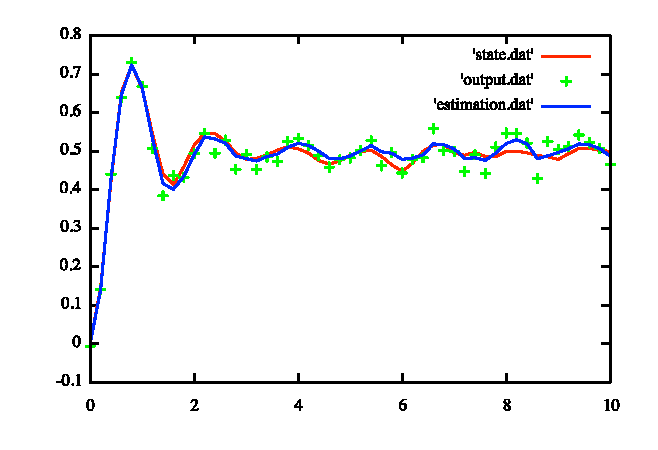
\includegraphics{ornstein}}
\end{ImageNoCaption}
\hypertarget{page2_sec3}{}\section{The CMakeList.txt}\label{page2_sec3}


\begin{DocInclude}\begin{verbatim}CMAKE_MINIMUM_REQUIRED(VERSION 2.6)

PROJECT(Van_Der_Pol)
ADD_DEFINITIONS(" -O3")

# GSL
SET(BFILT_LIB bfilt)

# Include et Link Directories

IF(APPLE)
  MESSAGE("-- Apple Configuration")
  INCLUDE_DIRECTORIES(
    /sw/include/
    )
ENDIF(APPLE)

# Executables and "stand-alone " librairies
ADD_EXECUTABLE (Van_Der_Pol
  van_der_pol.cpp
  example_3.cpp
  )

# Linkage
TARGET_LINK_LIBRARIES(Van_Der_Pol
  ${BFILT_LIB}     
  )
\end{verbatim}
\end{DocInclude}
 